%Esta es la sección resultados de programación de la aplicación.
A continuación se presentan los resultados obtenidos despues de haber implementado
las gramaticales y las funciones que se agregaron para dibujar las figuras solicitadas

\begin{lstlisting}
/**
 * Script para dibujar una casa y un carro simple.
 */
//Instrucciones para dibujar un carro
color 1;
rectangle 70 120 200 90;
rectangle 106 90 130 30;
color 2;
circle 156 230 50;
circle 236 230 50;

//Instrucciones para dibujar una casa
color 2;
rectangle 390 110 170 120;
rectangle 430 140 90 90;
color 3;
line 350 140 480 50;
line 480 50 600 140;
color 1;
circle 520 200 10;
\end{lstlisting}

La siguiente figura nos muestra el resultado de ejecutar las instrucciones mostradas 
previamente.

\begin{figure}[H]
	\begin{center}
		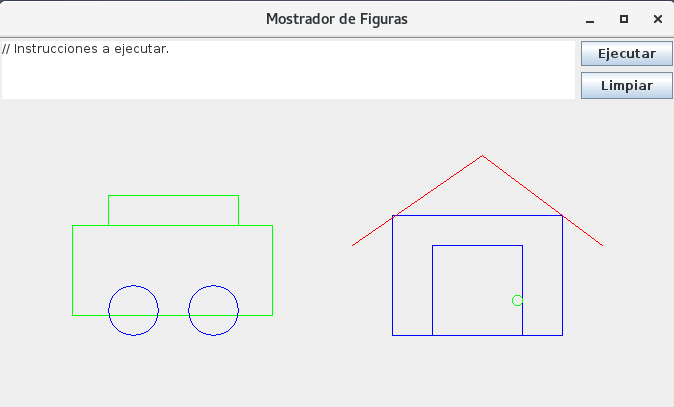
\includegraphics[scale=0.9]{images/img_ej_figs_awt}
		\caption{Operación de asignación de un vector a una variable de un sólo caractér.}
	\end{center}
\end{figure}

